%%%%%%%%%%%%%%%%%%%此部分为附录1环境代码,是比较笨的方法来适应论文撰写规范%%%%%%%%%%%%%%%%%%%%%%%%%%%%%%%%%%%%%%
%新增附录时只需要将\setcounter{chapter}{X}以及\chapter{附\texorpdfstring{\quad}{}录 X}中相应的X更改为相应的数字
\setcounter{chapter}{2} %从2开始编号
\setcounter{section}{0}
\setcounter{equation}{0}
\setcounter{table}{0}   
\setcounter{figure}{0}
\chapter{附\texorpdfstring{\quad}{}录 2} %附录2
%%%%%%%%%%%%%%%%%%%%%%%%%%%%%%%%%%%%%%%%%%%%%%%%%%%%%%%%%%%%%%%%%%%%%%%%%%%%%%%%%%%%%%%%%%%%%%%%%%%%%%%%
%%%%%%%%%%%%以下为用户代码,用于撰写您的论文%%%%%%%%%%%%%%%%%%%%%%%%%%%%%%%%%%%%%%%%%%%%%%%%%%%%%%%%%%%%%%

在论文撰写规范中,下面两段话让人费解:

\begin{enumerate}
	\item 	对需要收录于学位论文中但又不适合书写于正文中的附加数据、方案、资料、详细公式推导、计算机程序、统计表、注释等有特色的内容,可做为附录排写,序号采用“附录1”、“附录2”等。	
	\item	公式序号按章编排,如第一章第一个公式序号为“(1-1)”,附录2中的第一个公式为“(2-1)”等。
\end{enumerate}

论文撰写规范要求的附录和通常书籍上使用附录A、附录B等编号的不一样,上述要求最终的效果是这些编号容易和正文的混淆。特殊的要求和代码的耦合,使我不得不使用比较笨的方法来设计附录部分的模板。这部分还需要有附录需求的同学来完善,为了目录中美观且不命名冲突,还是不在附录使用图表。

\section{测试测试测试}
\subsection{测试测试测试}
%
测试测试测试测试测试测试测试测试测试测试测试测试
\begin{align}
\left\{\begin{array}{l}
\dot{v}_{1}(t)=v_{2}(t) \\
\dot{v}_{2}(t)=R^{2}\left(-\zeta_{1}\left[v_{1}(t)-v_c(t)\right]^{\alpha}-\zeta_{2}\left[\dfrac{v_{2}(t)}{R}\right]^{\beta}\right)
\end{array}\right.	
\end{align}
\begin{align}
\left\{\begin{array}{l}
\dot{v}_{1}(t)=v_{2}(t) \\
\dot{v}_{2}(t)=R^{2}\left(-\zeta_{1}\left[v_{1}(t)-v_c(t)\right]^{\alpha}-\zeta_{2}\left[\dfrac{v_{2}(t)}{R}\right]^{\beta}\right)
\end{array}\right.	
\end{align}
% 注释掉图表:
% \begin{figure}[htbp]
% 	\centering	
% 	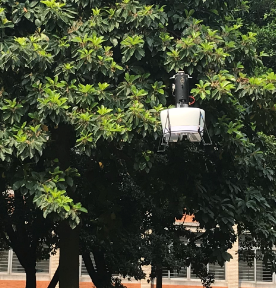
\includegraphics[scale=1]{Fig/DFUAV_f31.png}
% 	\caption{\label{fig_c1}测试测试测试}
% \end{figure}
% \begin{figure}[htbp]
% 	\centering	
% 	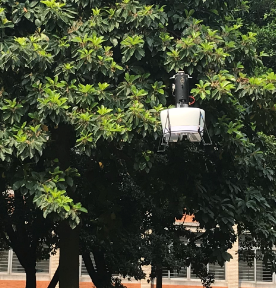
\includegraphics[scale=1]{Fig/DFUAV_f31.png}
% 	\caption{\label{fig_c2}测试测试测试}
% \end{figure}
% \begin{table}
% 	\caption{\label{DF_p1}测试测试测试}
% 	\centering{}%
% 	\small 
% 	\begin{tabular}{cccccc}
% 		\hline 
% 		参数符号 & 数值&参数符号 & 数值&参数符号 & 数值\tabularnewline
% 		\hline 
% 		$ A_x,A_y,A_z $  & $ 0.04082\,\text{m}^2 $ &$ \rho $        &$1.225\,\text{kg}/\text{m}^3$&$ I_b $           & $ 0.000029 $               \tabularnewline
% 		$ k_{\varpi} $   & $1.13342 \times 10^{-6}$& $ d_{\varpi} $ & $1.13342 \times 10^{-7}$ 	  &$k_{\delta} $     & $ 0.01495 $ 			      \tabularnewline
% 		$C_{D,x},C_{D,y}$& $ 0.43213 $             &$ C_{D,z} $     & $ 0.13421 $             	  &	$ q_a $ 	     & $ 1.49 $ 				  \tabularnewline
% 		$ l_{a} $        & $ -0.1121\,\text{m} $   & $ d_{ds} $     & $ 0.01495 $			  	  &$ d_{af} $        & $ 0.01495 $    			  \tabularnewline
% 		$ R $            & $ 0.11\,\text{m} $      &$ b $           & $ 2 $       			   	  &$ S $ 			 & $ 0.04082\,\text{m}^2 $    \tabularnewline
% 		$C_{l_{\alpha}}$ & $ 2.212\,/\text{rad} $  &$C_{l, \max } $ & $ 1.05 $ 				   	  &$ C_{l, \min } $  & $ -1.05 $ 				  \tabularnewline
% 		$ l_2 $          & $ 0.06647\,\text{m} $   &$ l_1 $         & $ 0.17078\,\text{m} $    	  &	$ m $ 		     & $ 1.53\,\text{kg} $ 		  \tabularnewline
% 		$ C_{d, o } $    & $ 0.9 $                 &$ C_{d, g } $   & $ 0.9 $					  &$ C_{duct} $      & $ 0.78497 $	 			  \tabularnewline
% 		$ I_x $          & $ 0.02548 $ 			   &$ I_y $         & $ 0.02550 $                 &$ I_z $			 & $ 0.00562 $ 				  \tabularnewline
% 		\hline 
% 	\end{tabular}	
% \end{table}

% \begin{table}
% 	\caption{\label{TDF_p2}测试测试测试}
% 	\centering{}%
% 	\small 
% 	%	\resizebox{\textwidth}{!}{
% 	\begin{tabular}{cccccc}
% 		\hline 
% 		参数符号 & 数值&参数符号 & 数值&参数符号 & 数值\tabularnewline
% 		\hline 
% 		$ I_x $ & $ 054593 $ &$ I_y $ & $ 0.017045 $& $ I_z$ & $ 0.049226 $ \tabularnewline
% 		$ l_{1} $ & $ 0.0808\,\text{m} $&$ l_{2} $ & $ 0.175\,\text{m} $ &$ l_3 $ & $ 0.06647\,\text{m} $ \tabularnewline 
% 		$ l_4 $ & $ 0.2415\,\text{m} $ &$ l_5 $ & $ 0.1085\,\text{m} $& $ m $ & $ 3.7\,\text{kg} $ \tabularnewline
% 		\hline 
% 	\end{tabular}	%}
% \end{table}